\documentclass{article}
\usepackage{tikz}
\usetikzlibrary{arrows,arrows.meta,automata,backgrounds,calc,patterns,positioning,shapes,shadows}
\pgfdeclarelayer{bg}
\pgfsetlayers{bg,main}
\tikzset{
	rv/.style={draw, ellipse},
	pf/.style={draw, rectangle, fill = gray!30},
	arc/.style = {->, >={[round,sep]Stealth}},
}

\newcommand{\factorat}[4]{
	\node[pf, label={#2:{#3}}](#4) at (#1) {};
}

\newcommand{\factor}[6]{
	\node[pf, #1=#3 of #2, label={#4:{#5}}](#6) {};
}

\begin{document}

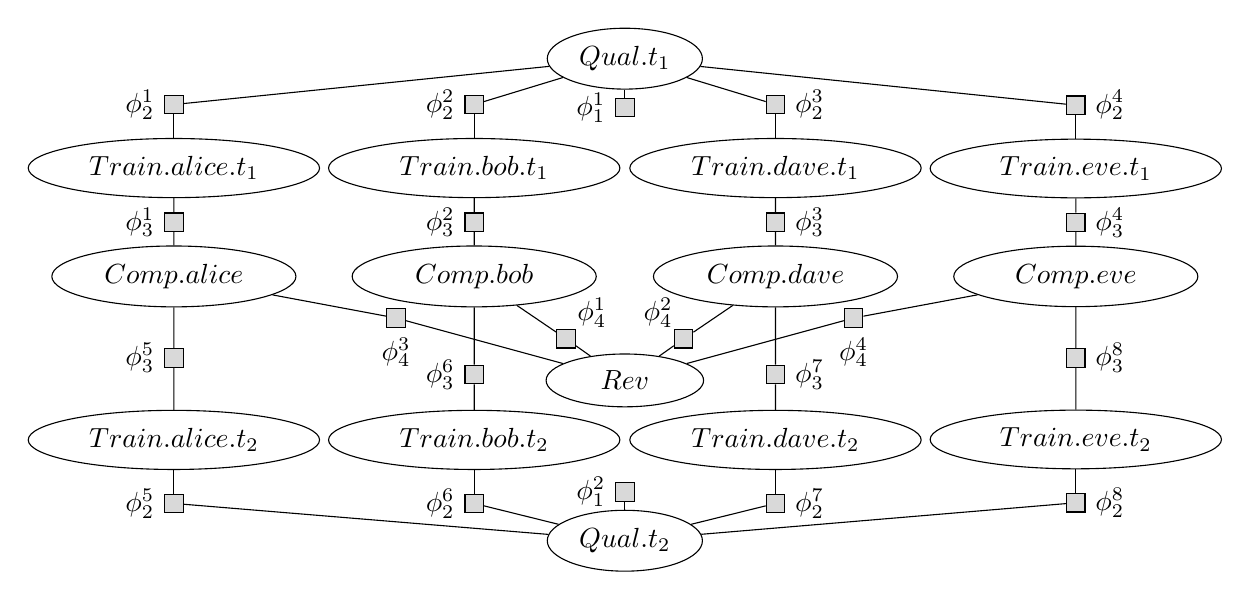
\begin{tikzpicture}
	\node[rv, draw, minimum width = 2.0cm] (rev) {$Rev$};
	\node[rv, draw, above left  = 0.8cm and 0.1cm of rev, minimum width = 3.1cm] (com_b) {$Comp.bob$};
	\node[rv, draw,       left  = 0.7cm of com_b,         minimum width = 3.1cm] (com_a) {$Comp.alice$};
	\node[rv, draw, above right = 0.8cm and 0.1cm of rev, minimum width = 3.1cm] (com_d) {$Comp.dave$};
	\node[rv, draw,       right = 0.7cm of com_d,         minimum width = 3.1cm] (com_e) {$Comp.eve$};

	\factorat{$(com_a.east)!0.4!(rev.west)$}{270}{$\phi_{4}^{3}$}{f1}
	\factorat{$(com_b.east)!0.6!(rev.west)$}{[label distance=-1.5mm]45}{$\phi_{4}^{1}$}{f2}
	\factorat{$(com_d.west)!0.6!(rev.east)$}{[label distance=-1.5mm]135}{$\phi_{4}^{2}$}{f3}
	\factorat{$(com_e.west)!0.4!(rev.east)$}{270}{$\phi_{4}^{4}$}{f4}

	\node[rv, draw, above = 0.6cm of com_a, minimum width = 3.7cm] (train_a1) {$Train.alice.t_1$};
	\node[rv, draw, below = 1.3cm of com_a, minimum width = 3.7cm] (train_a2) {$Train.alice.t_2$};
	\node[rv, draw, above = 0.6cm of com_b, minimum width = 3.7cm] (train_b1) {$Train.bob.t_1$};
	\node[rv, draw, below = 1.3cm of com_b, minimum width = 3.7cm] (train_b2) {$Train.bob.t_2$};
	\node[rv, draw, above = 0.6cm of com_d, minimum width = 3.7cm] (train_d1) {$Train.dave.t_1$};
	\node[rv, draw, below = 1.3cm of com_d, minimum width = 3.7cm] (train_d2) {$Train.dave.t_2$};
	\node[rv, draw, above = 0.6cm of com_e, minimum width = 3.7cm] (train_e1) {$Train.eve.t_1$};
	\node[rv, draw, below = 1.3cm of com_e, minimum width = 3.7cm] (train_e2) {$Train.eve.t_2$};

	\factorat{$(com_a)!0.5!(train_a1)$}{180}{$\phi_{3}^{1}$}{f5}
	\factorat{$(com_a)!0.5!(train_a2)$}{180}{$\phi_{3}^{5}$}{f6}
	\factorat{$(com_b)!0.5!(train_b1)$}{180}{$\phi_{3}^{2}$}{f7}
	\factorat{$(com_b)!0.6!(train_b2)$}{180}{$\phi_{3}^{6}$}{f8}
	\factorat{$(com_d)!0.5!(train_d1)$}{0}{$\phi_{3}^{3}$}{f9}
	\factorat{$(com_d)!0.6!(train_d2)$}{0}{$\phi_{3}^{7}$}{f10}
	\factorat{$(com_e)!0.5!(train_e1)$}{0}{$\phi_{3}^{4}$}{f11}
	\factorat{$(com_e)!0.5!(train_e2)$}{0}{$\phi_{3}^{8}$}{f12}

	\node[rv, draw, above = 3.35cm of rev] (qual_t1) {$Qual.t_1$};
	\node[rv, draw, below = 1.3cm of rev] (qual_t2) {$Qual.t_2$};

	\factor{below}{qual_t1}{0.1cm}{180}{$\phi_{1}^{1}$}{f13}
	\factor{above}{train_a1}{0.3cm}{180}{$\phi_{2}^{1}$}{f14}
	\factor{above}{train_b1}{0.3cm}{180}{$\phi_{2}^{2}$}{f15}
	\factor{above}{train_d1}{0.3cm}{0}{$\phi_{2}^{3}$}{f16}
	\factor{above}{train_e1}{0.3cm}{0}{$\phi_{2}^{4}$}{f17}

	\factor{above}{qual_t2}{0.1cm}{180}{$\phi_{1}^{2}$}{f18}
	\factor{below}{train_a2}{0.3cm}{180}{$\phi_{2}^{5}$}{f19}
	\factor{below}{train_b2}{0.3cm}{180}{$\phi_{2}^{6}$}{f20}
	\factor{below}{train_d2}{0.3cm}{0}{$\phi_{2}^{7}$}{f21}
	\factor{below}{train_e2}{0.3cm}{0}{$\phi_{2}^{8}$}{f22}

	\begin{pgfonlayer}{bg}
		\draw (com_a) -- (f1);
		\draw (com_b) -- (f2);
		\draw (com_d) -- (f3);
		\draw (com_e) -- (f4);
		\draw (f1) -- (rev);
		\draw (f2) -- (rev);
		\draw (f3) -- (rev);
		\draw (f4) -- (rev);
		\draw (train_a1) -- (f5);
		\draw (train_a2) -- (f6);
		\draw (train_b1) -- (f7);
		\draw (train_b2) -- (f8);
		\draw (train_d1) -- (f9);
		\draw (train_d2) -- (f10);
		\draw (train_e1) -- (f11);
		\draw (train_e2) -- (f12);
		\draw (f5) -- (com_a);
		\draw (f6) -- (com_a);
		\draw (f7) -- (com_b);
		\draw (f8) -- (com_b);
		\draw (f9) -- (com_d);
		\draw (f10) -- (com_d);
		\draw (f11) -- (com_e);
		\draw (f12) -- (com_e);
		\draw (qual_t1) -- (f13);
		\draw (qual_t1) -- (f14);
		\draw (qual_t1) -- (f15);
		\draw (qual_t1) -- (f16);
		\draw (qual_t1) -- (f17);
		\draw (train_a1) -- (f14);
		\draw (train_b1) -- (f15);
		\draw (train_d1) -- (f16);
		\draw (train_e1) -- (f17);
		\draw (qual_t2) -- (f18);
		\draw (qual_t2) -- (f19);
		\draw (qual_t2) -- (f20);
		\draw (qual_t2) -- (f21);
		\draw (qual_t2) -- (f22);
		\draw (train_a2) -- (f19);
		\draw (train_b2) -- (f20);
		\draw (train_d2) -- (f21);
		\draw (train_e2) -- (f22);
	\end{pgfonlayer}
\end{tikzpicture}

\end{document}